\chapter{Scripts}

This appendix chapter collects the example scripts used in this notebook.

\section{\textit{Vim} Configuration \texttt{vimrc} Used in Section \ref{ch:tfe}}

\begin{lstlisting}
call plug#begin()
Plug 'vim-airline/vim-airline'
Plug 'joshdick/onedark.vim'
call plug#end()

inoremap jj <Esc>
noremap j h
noremap k j
noremap i k
noremap h i

noremap s <nop>
noremap S :w<CR>
noremap Q :q<CR>

syntax on
colorscheme onedark

set number
set cursorline
set wrap
set wildmenu

set hlsearch
exec "nohlsearch"
set incsearch
set ignorecase
noremap <Space> :nohlsearch<CR>
noremap - Nzz
noremap = nzz

noremap sj :set nosplitright<CR>:vsplit<CR>
noremap sl :set splitright<CR>:vsplit<CR>
noremap si :set nosplitbelow<CR>:split<CR>
noremap sk :set splitbelow<CR>:split<CR>
noremap <C-j> <C-w>h
noremap <C-l> <C-w>l
noremap <C-i> <C-w>k
noremap <C-k> <C-w>j
noremap J :vertical resize-2<CR>
noremap L :vertical resize+2<CR>
noremap I :res+2<CR>
noremap K :res-2<CR>

set scrolloff=3
noremap sc :set spell!<CR>
\end{lstlisting}

\chapter{Continuous Integration and Delivery}

This notebook is mainly about Linux. In this appendix chapter, the boundary of the notebook is slightly expanded to software development, which is quite often how Linux is used in practice.

Continuous integration and delivery (CI/CD) is both a philosophical concept and a bunch of technology that speeds up the development, testing and deployment cycle of a software. It has become a common and beneficial practice that collaborative projects with rapid update implement the practice.

This chapter introduces CI/CD as well as tools to carry out CI/CD. In particular, GitHub, a widely appreciated CI/CD integrated platform to manage and share collaborative projects, is briefly introduced. The introduction of GitHub focuses on GitHub Action, the tool GitHub uses for CI/CD.

Some contents of this chapter come from \cite{honai2023cicd}.

\section{Agile VS Waterfall}

Agile and waterfall are both project management methodologies. Both of them are introduced starting with the more conventional waterfall model then Agile.

\subsection{Waterfall}

Speaking of project proposal, development, testing and delivery cycle, it is fairly intuitive to follow the procedures below:
\begin{enumerate}
	\item Understand requirements from the user.
	\item Design the architecture of the solution.
	\item Develop the solution.
	\item Test the solution.
	\item Deliver the solution and close the project.
	\item (Follow-up) maintain the solution.
\end{enumerate}
The philosophy behind waterfall, as its name indicates, is to ``follow the procedures and do not turn back''. When a previous step is considered completed, it is completed and should not be revoked or revised. This is demonstrated by Fig. \ref{ch:cicd:fig:waterfall}.
\begin{figure}[htbp]
	\centering
	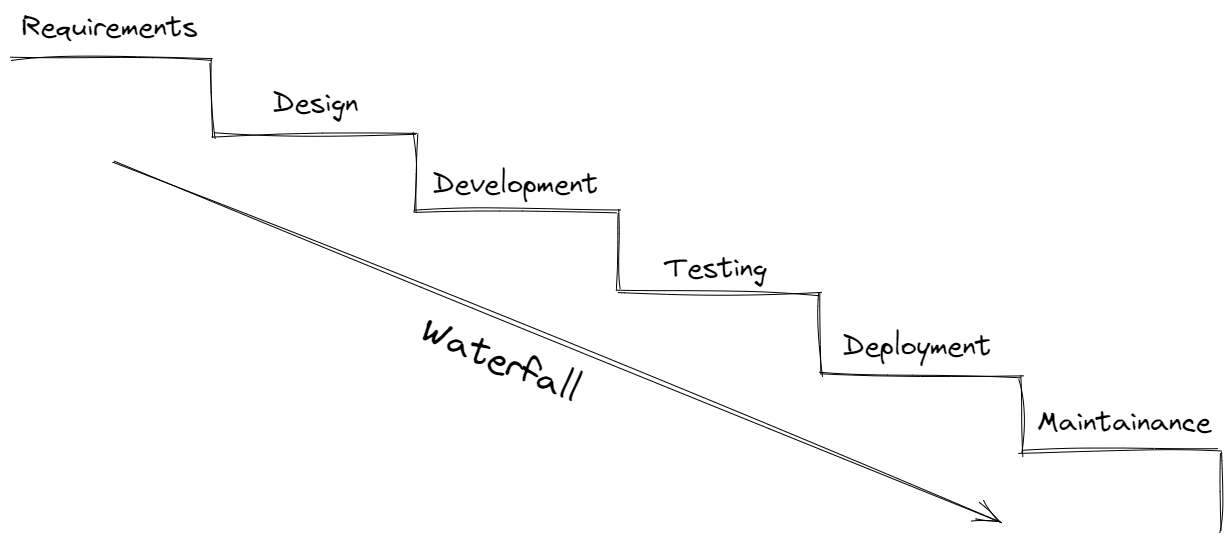
\includegraphics[width=300pt]{chapters/ap/figures/waterfall.png}
	\caption{Waterfall model.} \label{ch:cicd:fig:waterfall}
\end{figure}

With waterfall, a project can be designed, developed and deployed in a relatively efficient manner. However, there is one limitation: everything done in earlier steps cannot be changed in later steps. This sets up a high bar on both the user and the developer. For example, in step 1 ``understand requirements from the user'', the user needs to illustrate all the requirements to the developer as they cannot be modified in later steps. Similarly, in step 2 ``design the architecture'', the developer needs to optimize the design to his best, as the architecture cannot be changed later.

Regrettably, with the rapid change in the market and the aggressive advent in technology today, it is challenging even for the smartest user and developer to determine all the requirements and designs in the beginning stage of the project. More likely, the requirements of the user have to change align with the market trend, and so does the design of the solution.

For a new feature to be added into the existing system, it is possible to simply start a new project flow for the new feature, and integrate it into the existing system later. However, integrating the new feature into the existing system can also be challenging when the design is complicated and coupled. The integration often introduces a blackout period of the system. If the system is already deployed, the customer experience would be affected by the blackout.

\subsection{Agile}

Agile is the counterpart of waterfall. It is proposed to tackle the aforementioned issue: rapid change of requirements and adaptations to new technology and tools. It allows continuous integration and deployment of new features into the system in a convenient and systematic way, without introducing blackout.

In agile architecture, each feature is separately modularized. Each feature, before deploying and integrating into production environment, circulates in its own ``development and testing circle'', where it can be tested and reviewed iteratively by the developers and the users audit team, as shown below in Fig. \ref{ch:cicd:fig:agile}.
\begin{figure}[htbp]
	\centering
	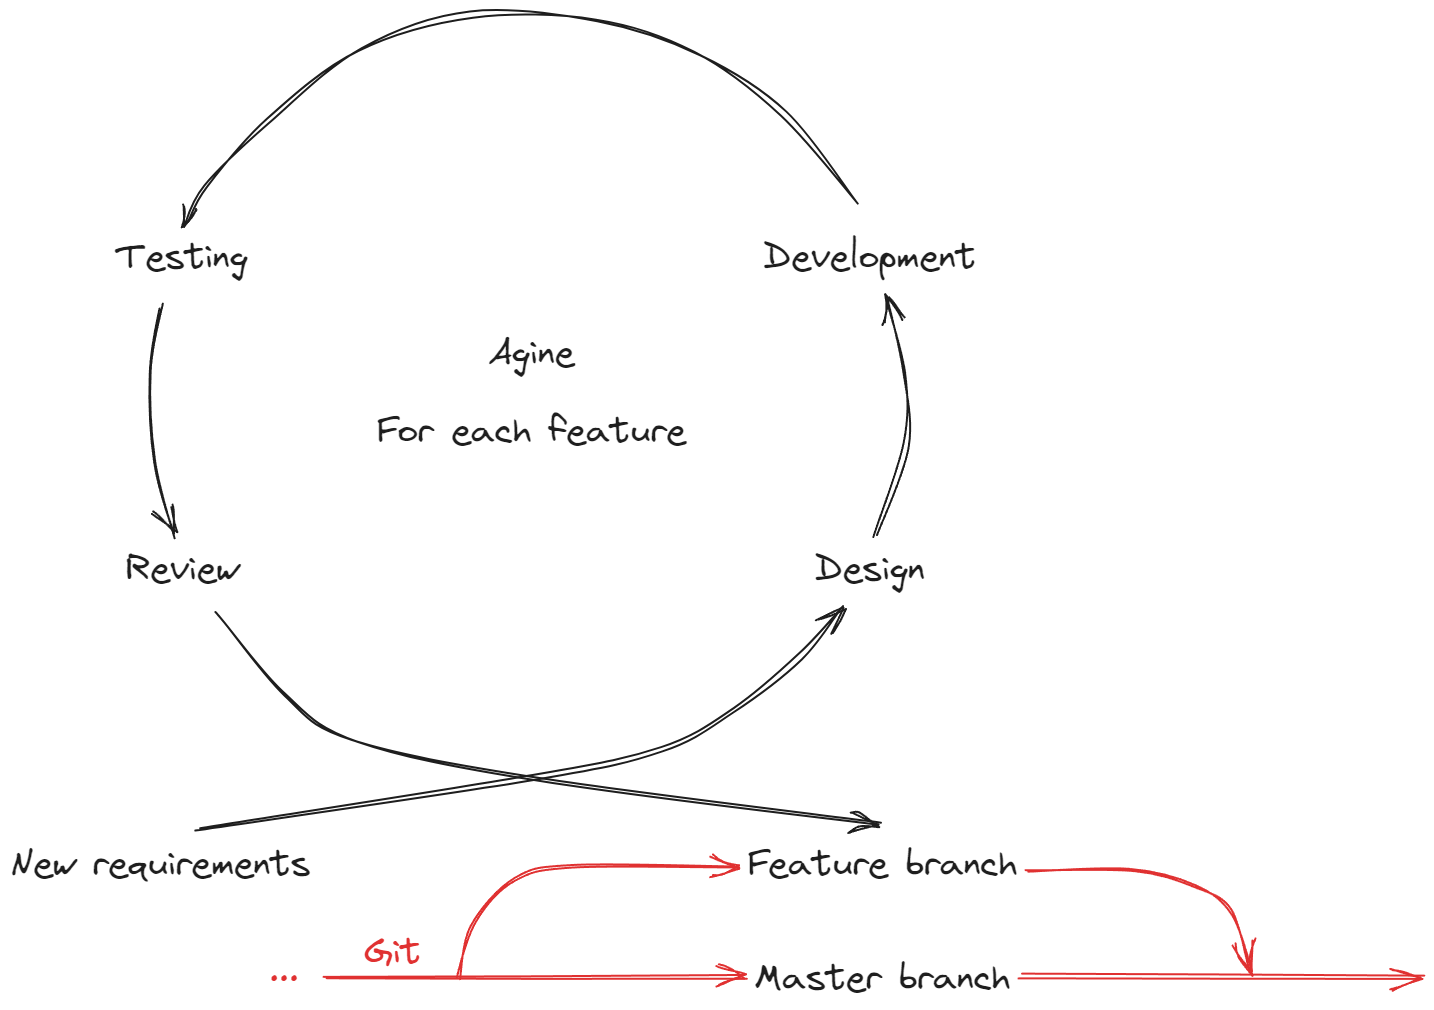
\includegraphics[width=300pt]{chapters/ap/figures/agile.png}
	\caption{Agile model.} \label{ch:cicd:fig:agile}
\end{figure}

Agile allows rapid change to be made to the requirements and realizations of a feature. Should there be a change, just keep cycling in Fig. \ref{ch:cicd:fig:agile} until the change is implemented and tested, before it is pushed back to the master branch.

In parallel development where there are multiple features running in their associated circles, the developer can easily choose which feature branch and circles to prioritize. This gives the developer a clearer overview of what is happening and how to best response to the customers immediate requirements.

\subsection{Roles in Agile-based Development}

The following roles are defined in agile, each role coming with a responsibility. The roles may slightly differ for each project. The most commonly seen approach, namely \textbf{scrum}, is introduced in Table. \ref{ch:cicd:tab:agilerole}.
\begin{table}[htbp]
	\centering
	\caption{Roles in Agile model.} \label{ch:cicd:tab:agilerole}
	\begin{tabularx}{\textwidth}{lX}
		\hline
		Role & Description \\
		\hline
		Product owner & Manage the entire program. He understands all the user requirements and progression of all features. He also signs off each feature when they are deployed. \\ \hdashline
		Scrum master & Lead the developer team as team manager or chief developer. \\ \hdashline
		Developer & Based on requirements, program the features. \\ \hdashline
		Tester & Design test cases to verify the efficacy of the developed feature. \\ \hdashline
		Operator/Supporter & Maintain the software \\
		\hline
	\end{tabularx}
\end{table}

In this role assignment, the product owner and scrum master come up with the product backlog, which clarify the sprints (tasks) and their priorities. The team then knows which sprints they shall work on first.

In the case where the features concerns a professional domain (such as economics, medical, etc.) that the developers cannot understand, business analysts are involved who bridge the user and the developer.

For each sprint, sprint planning and sprint backlog are proposed that describes the schedule of the sprint. The team works on the sprint and host daily scrum meetings until the sprint is solved. Upon finishing of a sprint, sprint review is hosted for audition.

\section{Continuous Integration Continuous Delivery}

CI/CD is introduced in this section. As a start, pipeline is introduced. Pipeline is an important concept used in CI/CD.

\subsection{Pipeline}

Pipeline is a set of data processing elements in a queue, where the output of the upper stream process is the input of the down stream process. An example is shown in Fig. \ref{ch:cicd:fig:pipeline}. By using a pipeline and let multiple pipelines at different execution phase run in parallel, the efficiency of the system is increased.
\begin{figure}[htbp]
	\centering
	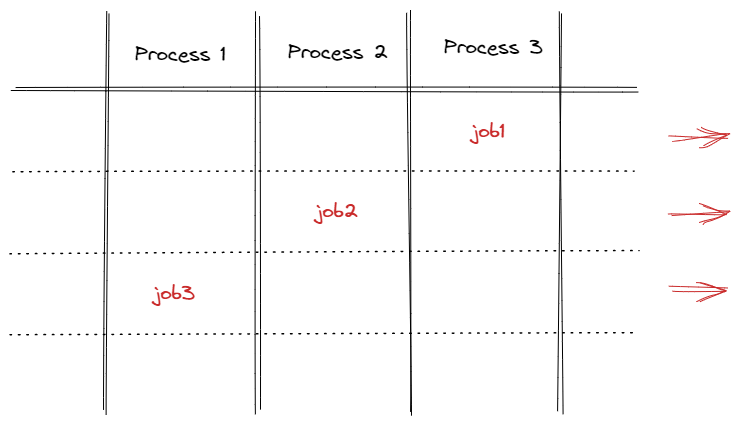
\includegraphics[width=300pt]{chapters/ap/figures/pipeline.png}
	\caption{Pipeline.} \label{ch:cicd:fig:pipeline}
\end{figure}

Pipeline is widely used in OS for process and thread management (recall Fig. \ref{ch:pm:fig:processflow}). It is also used in CI/CD.

\subsection{Continuous Integration}

In the development of a sprint, new codes are rapidly developed, and they are rapidly compiled, packaged and tested.

Conventionally, the integration of a new feature requires involvement from multiple parties. An example is given in Fig. \ref{ch:cicd:fig:conventionalintegration}. It includes the developer who program the software following users (or business analysts) requests, the integration team who integrates the new feature with the existing system and compile the code into packages, and the operations team who upload the new system into the pre-prod environment for real data testing, and the testers who audit the output of the program running in the pre-prod environment.

Should there be any error along the way, the code is roll back the developer team for trouble shooting. When the new system with the updated code survives pre-prod environment, it is then pushed to the production environment.
\begin{figure}[htbp]
	\centering
	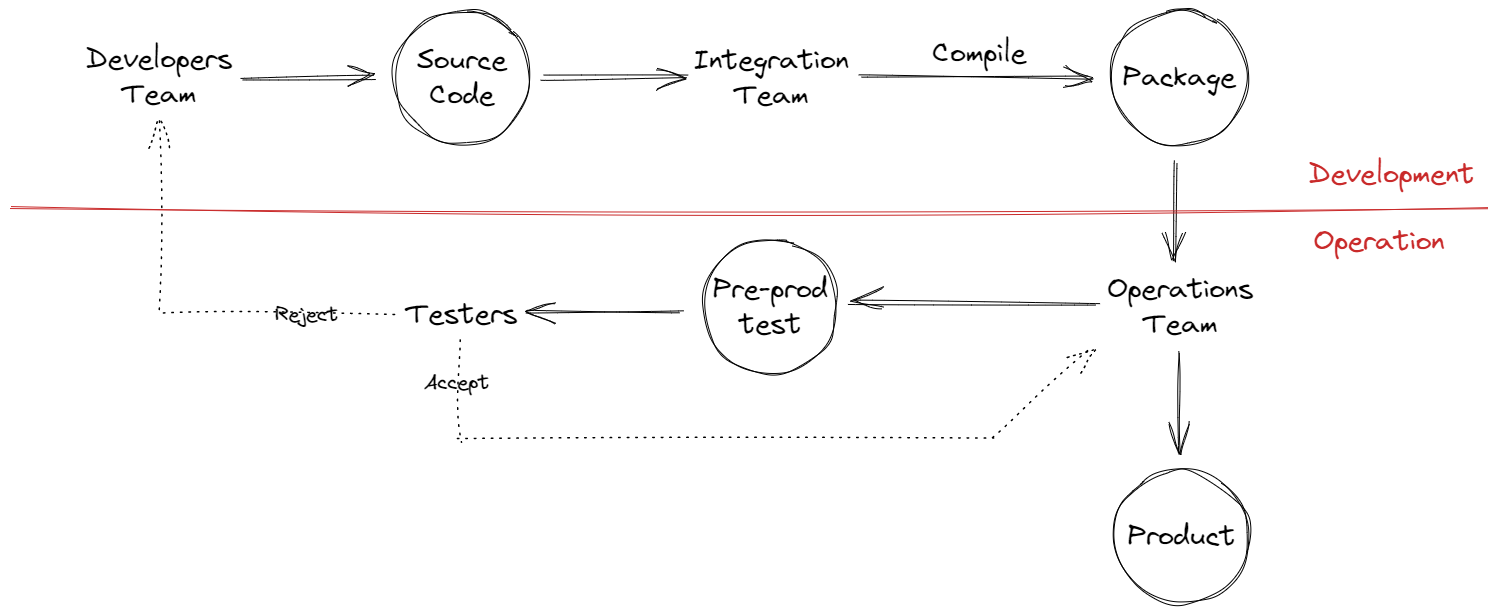
\includegraphics[width=350pt]{chapters/ap/figures/conventionalintegration.png}
	\caption{CI of a new feature.} \label{ch:cicd:fig:conventionalintegration}
\end{figure}

In practice, each cycle in Fig. \ref{ch:cicd:fig:conventionalintegration} can take a few days or even weeks as so many teams have to cooperate to make it happen. It takes time for the integration team to integrate different branches in the source code together, making sure that components from different branches function properly. When there is a defect, the flaws can be spotted only in the last stage of the iteration, i.e., testing. This practically disallows very frequent update of the system in response to the rapid changes in requirements.

CI (together with CD which is introduced in later section) tries to solve the above problems. CI automates the ``development'' portion in Fig. \ref{ch:cicd:fig:conventionalintegration}, while CD automates the ``operation'' portion.

To speed up the development of new features, CI mainly adopts the following methods.
\begin{itemize}
	\item Use \textit{Git} to manage features. This simplifies the procedure of managing multiple under-development features and integrating them together. Integration is now managed by \textit{Git} following developers' intention.
	\item Use a build server to automatically compile the code into ready-for-delivery packages. The scrum master and senior developers can access the server and monitor the progression. Should there be a compiling error, the developer is notified immediately.
	\item The code, after compiling, is immediately tested in the build server using pre-defined test cases. If the code fails the test cases, the developer is immediately notified.
\end{itemize}

CI effectively removed ``integration team'' from the picture. The integration related tasks are split into small pieces and processed by automation tools, feature integration by \textit{Git}, and compiling by build server. During CI, the developer not only generates the codes, but also supervises \textit{Git} and build server. Should there be any error, the developer is notified immediately by the automation tools.

CI speeds up the developing cycle, from the receiver receiving requests from the user, to the point they have new system in the package ready for pre-prod testing.

\subsection{Continuous Delivery}

The package received from the development side contains the latest version of the system where a new feature is integrated. It is, however, not certain at this point whether the new feature works properly and how the system would behave as a whole with this new feature. The sophisticated testing and deployment of the software features are done by the operations team.

Conventionally, operations team and the testers receive the updated package together with an instruction from the developers team. The instruction describes how the package shall be installed, and what test cases to use for auditing. The operations team and the testers need to understand the instructions, and configure the pre-prod environment accordingly for the testing. The testers then uses varieties of scenarios to test the performance of the software. Bugs, if any, are reported to the developers team. If no bugs are spotted, the testers notify the operation team to release the package into production environment.

There are some obvious drawbacks to the conventional approach. The developers team needs to give detailed and precise instruction to the operations team, and the developers may make mistakes or missing something in the instruction, especially regarding environment configuration. Besides, there are too many human interactions, which slow down the process and generates human error. The entire procedure usually take about a whole day.

CD is a software development practice that allows software to be released to production at any time. The idea behind CD is to deploy the code for testing automatically anytime CI provides a new package by adopting the following methods.
\begin{itemize}
  \item Use machine-readable instruction files for packages installation, and let the server virtualize the execution environment and install the packages automatically.
  \item Use machine-readable testing scripts, and let the server execute tests and analyze the results automatically.
  \item The aforementioned machine-readable instruction files and testing scripts are managed the same way as the source code by the developers.
\end{itemize}

Ideally, as soon as a version of packages is released by CI, CD can automatically have it deployed and tested, and return the testing results to CI without human interaction. This is shown by Fig. \ref{ch:cicd:fig:cd}. In this CI/CD implementation, the developer is playing a more comprehensive role than what is shown in Fig. \ref{ch:cicd:fig:conventionalintegration}.
\begin{figure}[htbp]
	\centering
	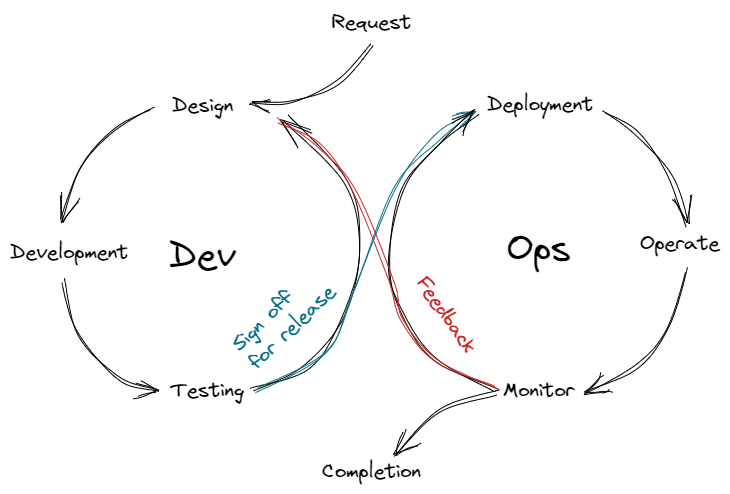
\includegraphics[width=350pt]{chapters/ap/figures/cd.png}
	\caption{CI and CD.} \label{ch:cicd:fig:cd}
\end{figure}

Under the framework of CI/CD in Fig. \ref{ch:cicd:fig:cd}, the developer not only develops the new feature, but also integrates the features with the help of version control and branch management tool \textit{Git}, compiles the packages using build server, deploys the new packages in the testing environment by preparing machine-readable instruction files, and finally tests the new features using pre-configured test cases in the machine-readable testing scripts.

Since the operation team joins the developers team, they are now called the DevOps team. The CI/CD framework shown in Fig. \ref{ch:cicd:fig:cd} is known as the CI/CD pipeline which represents an end-to-end software development lifecycle (SDLC) within its ecosystem.

This CI/CD framework enables fast deployment of new packages. Large IT companies can make up to dozens of new releases everyday.

\section{\textit{GitHub} Action (Part I: Basics)}

\textit{GitHub} has been an amazing platform for managing software projects, especially open-source collaborative projects.

In the early days when CI/CD was not enabled in \textit{GitHub}, developers used third-party CI/CD tools such as Jenkins and Travis CI in conjunction with \textit{GitHub} for automatic integration and deployment. Lately, \textit{GitHub} introduced \textit{GitHub} Action (for short, Action), its own CI/CD solution, as a response to developers' requests.

Action is the practice of CI/CD on GitHub. In short, it allows the developers to create automatic workflows tied to \textit{GitHub} events. Action is widely used to automate the following tasks:
\begin{itemize}
  \item Compile the source code. The developer can define how the source code should be compiled.
  \item Virtualize the environment to run the compiled packages. The developer can define how to set up the environment.
  \item Test the packages on testing scenarios. The developer can define the testing scenarios.
\end{itemize}
Machine-readable instruction files are used to guide the automation. They are managed together with the source code in the repository.

Notice that Action might be chargeable for private repositories depending on its computational cost. It is, however, often free of charge for community and public repository projects.

A commonly used scenarios of Action for community projects is that when someone submits a pull request, a series of checks are automatically done, and emails are sent to the project maintenance team to notify them the request. Sometimes a ``thank you'' email is sent to the contributor.

\begin{mdframed}
	\centerline{\textbf{Pull Request}}
	
	When an individual developer wants to contribute to an open-source community project of others, the following is the general flow.
	\begin{enumerate}
		\item The developer forks the project to his own \textit{GitHub} account.
		\item The developer clones a copy of the project from his own \textit{GitHub} account to his own machine.
		\item The developer creates a new branch about the feature he wants to add or improve.
		\item The developer develops the feature on the branch.
		\item The developer commits the development and pushes the commit to the forked repository.
		\item The developer submits a pull request to the maintenance team of the community project.
		\item The maintenance team receives the pull request and review the changes made to the code in the developer's forked repository.
		\item If no objection, the maintenance team pull the changes from the developer's forked repository, and merge the new feature branch with the existing branches.
	\end{enumerate}
	With the above, the developer becomes an official contributor to the community project.
\end{mdframed}

Another use case for Action for individual projects is that when a new code is pushed to the repository, the code is automatically compiled and tested. If the test returns an error, create a \textit{GitHub} issue. Otherwise, put out a new release.

\subsection{Framework}

In Action, the developer needs to prepare CI/CD pipelines known as workflows, either by himself or from Actions Marketplace (a platform where commonly used workflows are shared). The backbone of a workflow is YAML files that describe the environment, the trigger, and the list of actions to execute. When an event such as a pull request happens, the associated workflow is triggered and executed. A demonstrative plot is given in Fig. \ref{ch:cicd:fig:actionframework}.
\begin{figure}[htbp]
	\centering
	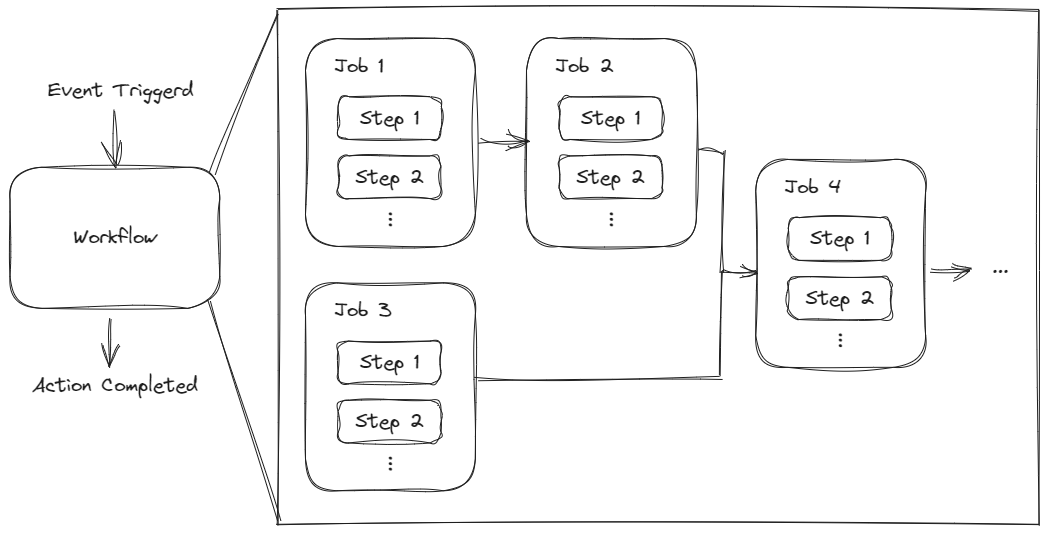
\includegraphics[width=350pt]{chapters/ap/figures/action_framework.png}
	\caption{Action framework.} \label{ch:cicd:fig:actionframework}
\end{figure}

As illustrated in Fig. \ref{ch:cicd:fig:actionframework}, a workflow can contain multiple jobs that can run in parallel (by default) or sequence (by defining dependencies). Each job can contain multiple steps that run in sequence.

For each job, a ``runner'' is assigned which serves as the environment to run the job. The developer needs to specify how the runner should be configured such as what software needs to be installed in order to run the associated job.

\subsection{Action Triggers and Types}

It is worth mentioning that Action can be triggered not only by \textit{GitHub} events but also external events, schedules, etc. Commonly seen triggers include
\begin{itemize}
	\item \textit{GitHub} Events, such as push, pull request, etc. This is the most common setup for CI/CD.
	\item External events.
	\item Schedule.
	\item Manual.
\end{itemize}

Action provides workflow templates of different task types. There are at least the following workflow types as of this writing. They are not limited to CI/CD.
\begin{itemize}
	\item CI
	\item Deployment
	\item Testing
	\item Code quality
	\item Code review
	\item Dependency management
	\item Monitoring
	\item Automation
	\item Utilities
	\item Pages
	\item Hugo
\end{itemize}
Some of them will be covered in later sections.

\subsection{Action Marketplace}

Action marketplace provides commonly seen actions for free, and they can be easily integrated into a workflow. The developer can look for action items in Action marketplace before trying to prepare the entire workflow by himself from scratch.

\subsection{Costs}

Action may generates additional costs. This is because executing workflows usually consumes \textit{GitHub} servers' storage and CPU. As of this writing, additional cost is generated only if all the following criteria are met:
\begin{itemize}
	\item Private repository. This is often not the case for community and individual projects, but often true for enterprise repositories.
	\item The workflows are executed on \textit{GitHub} servers. Notice that it is possible to execute workflows using on-premises servers, in which case Action becomes a free service.
	\item Storage and/or computational cost goes beyond the free-tier threshold.
\end{itemize}

When all the criteria is met, the developer pays \textit{GitHub} by the storage and computational consumption. He can select either prepaid mode (fixed bill, limited consumption per month) or postpaid mode (unfixed bill, unlimited consumption per month).

The running environment also affects the cost. It is often more expensive if the workflow needs to run on Windows or MacOS than if it can run on Linux due to the licensing fee. As of this writing, Windows and MacOS introduce a computational cost multiplier of $2$ and $10$ respectively comparing with Linux.

\section{\textit{GitHub} Action (Part II: Practice)}

As introduced in the previous section, the key to an Action includes defining the triggers and preparing the associated workflows for the triggers. Of course, the developer also needs to map the triggers with the workflows. More details are introduced in this section.

The workflow files are used to define the triggers as well as the associated workflows. They are YAML format files following specific syntax that illustrates environment configurations requirements, jobs, and job steps. They are stored under \verb|.github/workflows| and are managed by the developers just like any other source code. Notice that there are certain events that would trigger only if their associated workflow files exist in the project repository default branch (usually \verb|main| or \verb|master| branch).

As an example, here is a piece of workflow file from \textit{GitHub} document. \label{code:githubactionsdemo}
\begin{lstlisting}
name: GitHub Actions Demo
run-name: ${{ github.actor }} is testing out GitHub Actions
on: [push]
jobs:
  Explore-GitHub-Actions:
    runs-on: ubuntu-latest
    steps:
      - run: echo "The job was automatically triggered by a ${{ github.event_name }} event."
      - run: echo "This job is now running on a ${{ runner.os }} server hosted by GitHub!"
      - run: echo "The name of your branch is ${{ github.ref }} and your repository is ${{ github.repository }}."
      - name: Check out repository code
        uses: actions/checkout@v4
      - run: echo "The ${{ github.repository }} repository has been cloned to the runner."
      - run: echo "The workflow is now ready to test your code on the runner."
      - name: List files in the repository
        run: |
          ls ${{ github.workspace }}
      - run: echo "This job's status is ${{ job.status }}."
\end{lstlisting}

For the convenience of the reader, here is a brief introduction of YAML syntax.

\begin{mdframed}
\centerline{\textbf{YAML Syntax}}

YAML shares a lot of similarities with JSON. It is essentially a ``dictionary of dictionary'' document storage of information. The stored item under each field can be a string (can span multiple lines), a dictionary, or a list of items where each item can again be a string, a dictionary or a list of items.

For example, to store the basic information of a person in YAML, one may consider using
\begin{lstlisting}
name: Tom
job: developer
address: 1 Christmas Road
hobby: table tennis
\end{lstlisting}
where in this example all the items are single-line strings. This is the most simple implementation of YAML. Notice that space is allowed in both keys and values. However, it is not recommended to use spaces in keys as it is inconsistent with other languages.

Consider items that are dictionaries. For example, in the earlier example, the address may contain two fields, unit number and street name. In that case, use indent to represent dictionary layer as follows.
\begin{lstlisting}
name: Tom
job: developer
address:
  unit: 01-01
  street: Christmas Road
hobby: table tennis
\end{lstlisting}

Consider items that are lists. For example, in the earlier example, the person has multiple hobbies as follows.
\begin{lstlisting}
name: Tom
job: developer
address:
  unit: 01-01
  street: Christmas Road
hobby:
  - table tennis
  - football
\end{lstlisting}

Consider items that are list of dictionaries. For example, in the earlier example, the person has multiple addresses, each address represented by a dictionary containing unit and street information as follows.
\begin{lstlisting}
name: Tom
job: developer
address:
  - house_1:
      unit: 01-01
      street: 1 Christmas Road
  - house_2:
      unit: 09-27
      street: 127 Bell street
hobby:
  - table tennis
  - football
\end{lstlisting}

Though less common, there are alternative ways to represent dictionary and lists which look more like JSON as follows.
\begin{lstlisting}
name: Tom
job: developer
address: [house_1: {unit: 01-01, street: 1 Christmas Road}, house_2:{unit: 09-27, street: 127 Bell street}]
hobby: [table tennis, football]
\end{lstlisting}

To span a string in multiple lines, use the following
\begin{lstlisting}
address: |
  01-01
  1 Christmas Road
\end{lstlisting}
which includes the new line markers, and as a result the record in the above example would be a two-line string as seen, and
\begin{lstlisting}
address: >
  01-01
  1 Christmas Road
\end{lstlisting}
which excludes the new line markers, and as a result it is equivalent to
\begin{lstlisting}
address: 01-01 1 Christmas Road
\end{lstlisting}

Finally, YAML allows comments that start with \verb|#|.

In general, YAML is similar with JSON, but more human-readable and supports additional features such as string spanning and comments.

\end{mdframed}


\subsection{Trigger}

It is most common that an event triggers a workflow. An event can be defined in several ways such as
\begin{itemize}
	\item A person or a process does some operations to the \textit{GitHub} repository, such as submitting a pull request or pushing a new commit to the repository.
	\item Something happened outside \textit{GitHub} which serves as an external trigger that triggers a workflow.
	\item A schedule that runs a workflow at particular timestamps or periodically.
	\item Manually starting a workflow.
\end{itemize}

In a workflow YAML file, the trigger is defined by keyword \verb|on|. For example, one may see
\begin{lstlisting}
on:
  push:
    <...>	
\end{lstlisting}
or
\begin{lstlisting}
on:
  pull_request:
    <...>	
\end{lstlisting}
or
\begin{lstlisting}
on:
  scheduled:
    <...>	
\end{lstlisting}
which define different trigger types. It is possible to include multiple trigger types in the statement using a list, such as
\begin{lstlisting}
on:
  [push, pull_request]:
    <...>	
\end{lstlisting}

\subsection{Workflow}

A workflow contains multiple jobs that run in parallel or in sequence. A job contains multiple steps executed in sequence. Each step is something like a line of command in shell.

Each job is associated with a ``runner'' which is a physical or a virtual computer or container that execute the job. All the steps defined under a job need to run in the same environment. Of course, each step can call a different software program.

The following is an example given by \textit{GitHub} starter workflows template. Upon pushing a new commit, the workflow create a \textit{ubuntu} environment, install conda, python and associated packages, and finally run \verb|pytest| to check the code quality. \label{code:pythonpackageusingconda}
\begin{lstlisting}
name: Python Package using Conda
on: [push]
jobs:
  build-linux:
  runs-on: ubuntu-latest
  strategy:
    max-parallel: 5
  steps:
    - uses: actions/checkout@v3
    - name: Set up Python 3.10
      uses: actions/setup-python@v3
      with:
        python-version: '3.10'
    - name: Add conda to system path
      run: |
        # $CONDA is an environment variable pointing to the root of the miniconda directory
        echo $CONDA/bin >> $GITHUB_PATH
    - name: Install dependencies
      run: |
        conda env update --file environment.yml --name base
    - name: Lint with flake8
      run: |
        conda install flake8
        # stop the build if there are Python syntax errors or undefined names
        flake8 . --count --select=E9,F63,F7,F82 --show-source --statistics
        # exit-zero treats all errors as warnings. The GitHub editor is 127 chars wide
        flake8 . --count --exit-zero --max-complexity=10 --max-line-length=127 --statistics
    - name: Test with pytest
      run: |
        conda install pytest
        pytest

\end{lstlisting}

This workflow example defines one job, \verb|build-linux|. The job defines five steps, \verb|Set up Python 3.10|, \verb|Add conda to system path|, \verb|Install dependencies|, \verb|Lint with flake8| and \verb|Test with pytest|. Each step is associated with one \verb|run| that executes a command in the shell, for example,
\begin{lstlisting}
name: Install dependencies
run: conda env update --file environment.yml --name base
\end{lstlisting}
executes a \verb|conda| command that updates the packages defined in \verb|environment.yml| in the base environment.

In this example, it can be seen that many things besides the commands are configured in the workflow, such as the name of the jobs and steps, the OS, the Action reference, the software version, etc.

Notice that \verb|uses: actions/checkout@v3| as the first step in the list of steps pulls in a predefined action defined at \textit{github.com/actions/checkout}. The domain name \textit{github.com/} can be neglected.

Further details can be configured that are not shown in this example. Just to give one example, by using
\begin{lstlisting}
on:
  push:
    branches:
      - main
      - branch-1
      - branch-2
\end{lstlisting}
it can be specified which branch(es) to trigger the workflow when push a commit.

\subsection{Execution}

The workflow file needs to be saved under \verb|.github/workflows/| in the repository, with an arbitrary name but it has to end with suffix \verb|.yml| or \verb|.yaml|.

Push the repository with the workflow file to \textit{GitHub}. On \textit{GitHub} repository dashboard under ``Action'', select and enable the action so that the workflow would be triggered once the trigger event occurs.

\subsection{Very Complicated Actions}

Some Action workflows can be as simple as a few lines of shell commands, for example, \verb|GitHub Action Demo| given on page \pageref{code:githubactionsdemo}. Others, however, can be extremely complicated that includes a large set of implementation code, test cases, building, checking for vulnerabilities, packaging, etc. An example of such complicated Action flow is \verb|actions/checkout@v3| which was used in the other example \verb|Python Package using Conda| given in page \pageref{code:pythonpackageusingconda}.

More details of the action can be found at \textit{github.com/actions/checkout}. As of this writing, the latest version of the code is \verb|v4.1.0|, and in its repository it has a long list of files in TypeScript (an enhanced superset of JavaScript), YAML, JSON, shell scripts and other languages, and it is still under development. A screenshot is given in Fig. \ref{ch:cicd:fig:actioncheckout}.
\begin{figure}[htbp]
	\centering
	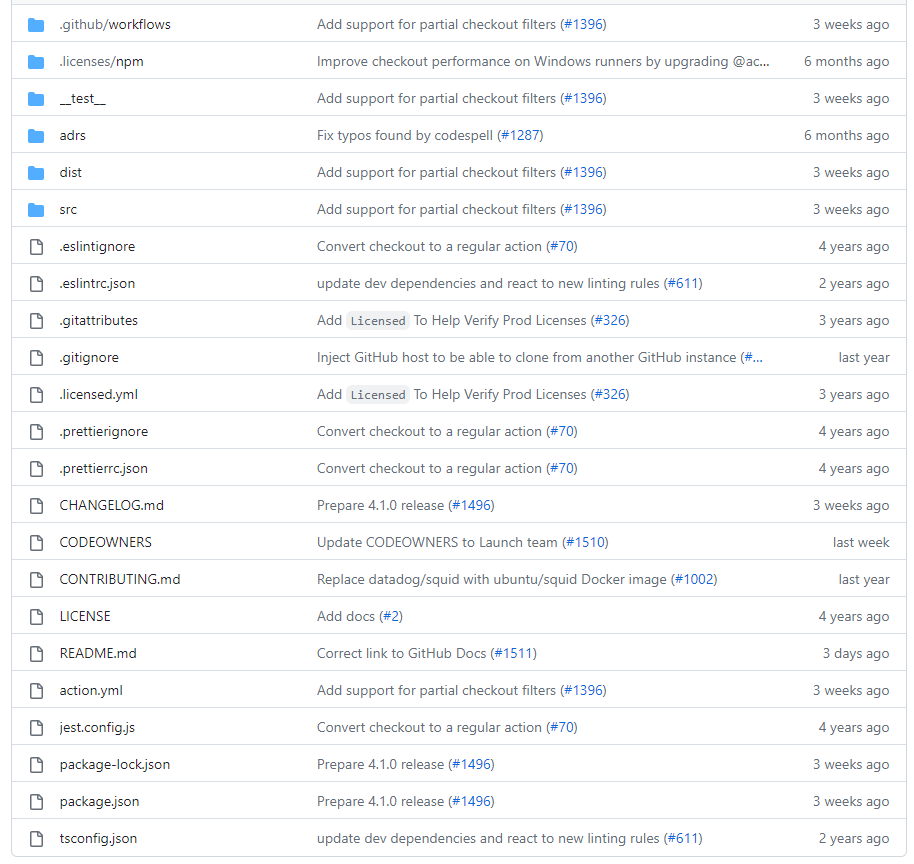
\includegraphics[width=350pt]{chapters/ap/figures/action_checkout.png}
	\caption{CI and CD.} \label{ch:cicd:fig:actioncheckout}
\end{figure}
Like other actions, it stores the workflow files (for this action, there are many of them) under \verb|.github/workflows|. The scripts that does all the actual jobs, in this action, are written in TypeScript and are stored under \verb|src|. Supporting materials such as license, reference to contributors, etc., are also included.

To package such a complicated action, there must be an \verb|action.yml| or \verb|action.yaml| that contains metadata of the action. This file specifies the inputs, outputs and configurations of the action.

It would be too detailed to go through all the files in \textit{github.com/actions/checkout}. The message here is that an action can be designed to be very complicated and powerful.































